  
  \smod je distribuován pod GPL licencí, takže uživatel má dvě možnosti jak získat model \smod: jako zdrojový kód a jako binární knihovnu. 
  
  Na stránkách katedry ... \pozn{dopln} lze stáhnout aktuální zdrojový kód modelu. Na stránkách github.com ... \pozn{dopln} lze stáhnout aktuální zdrojový či vývojové vrze. Na stránkách github.com ... \pozn{dopln}  lze rovněž stáhnout zdrojový kód toho manuálu. 
  
  Druhou možností je stáhnuté spustitelného instalačního souboru. Tento soubor je k dispozici ke stažení na odkazu ...\pozn{dopln}. Po spuštění toto souboru se spustí průvodce k instalaci standardního balíčku Python (úvodní obrazovka průvodce je ukázána na obrázku~\ref{fig:pruvodce}). Po ukončení instalace lze model \smod importovat do Python skriptu příkazem {\tt import smoderp2d}. 

  Před použitím modelu se doporučuje provést test, který ověří zda má uživatel nainstalované ostatní balíčky, které model \smod používá. Testovací skript je spolu s testovacími daty ke stažení na adrese ...\pozn{adresa dopln}. Testovací skript s názvem {\tt importrun.py} uložte do společné složky s testovacími daty {\tt test-data}. Po spuštění skripty se otevře okno terminálu příkazové řádky. Pokud instalace malíčku \smod neproběhla nebo proběhla chybně vypíše testovací skript hlášení ukázané na obrázku~\ref{fig:importerror}. Pokud nainstalované jiné nezbytné může se chybové hlášení lišit. Pokud například chybí balíček {\tt numpy} vypadá třetí řádek hlášení následovně: {\tt No module named numpy}. V takovém případě je nutné chybějící balíčky doinstalovat běžným způsobem. Pokud proběhne testovací běh modelu \smod bezchybně, proběhne v okně terminálu hlášení ukázané na obrázku~\ref{fig:testok}. Výstupní soubory jsou pak uložený do stejného adresáře do složky {\tt test-out}. V tento moment je model \smod a nezbytné malíčky zdárně nainstalovaný a je připraven k použití.
  
  \begin{figure}[b!]
    \centering
    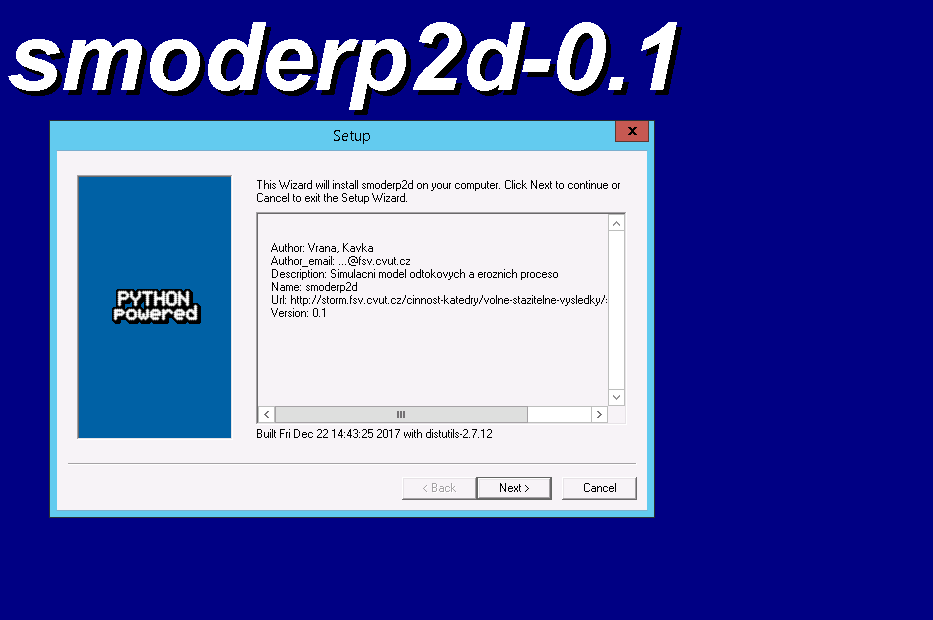
\includegraphics[width=0.75\textwidth]{./img/instalace.png}
    \caption{Úvodní obrazovka při instalaci malíčku \smod}
    \label{fig:pruvodce}
  \end{figure}
% 
  \begin{figure}[b!]
    \centering
    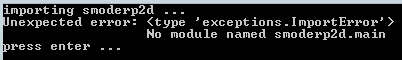
\includegraphics[width=0.75\textwidth]{./img/importerror.png}
    \caption{Hlášení při chybné instalaci malíčku modelu \smod}
    \label{fig:importerror}
  \end{figure}
% 
  \begin{figure}
    \centering
    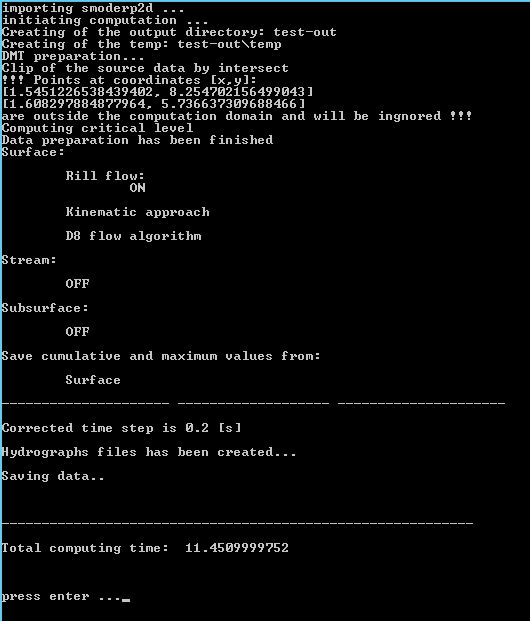
\includegraphics[width=0.75\textwidth]{./img/testok.png}
    \caption{Zdárný průběh testovacího skriptu modelu}
    \label{fig:testok}
  \end{figure}
  
\subsection{Použití modelu v ArcGIS}
  
  Současná verze modelu \smod využívá k přípravě vstupních dat výhradně software ArcGIS a Python malíčkem {\tt arcpy}. Proto je potřeba vytvořit skript, který načte s spustí model \smod. Takoví skript (s názvem {\tt start-smoderp2d.py}) může vypadat následovně:
  \begin{lstlisting}
    import smoderp2d.main as sm
    sm.run()
  \end{lstlisting}
  
  Následně je třeba vytvořit ArcGIS {\tt toolbox}, kde je soubor {\tt start-smoderp2d.py} nastavený jako zdrojový (obrázek~\ref{fig:tbsource}). Další krok je nastavení parametrů ArcGIS {\tt toolbox} odkud se načítají. Pořadí zadávaných hodnot je nutné dodržet. Ukázka ArcGIS {\tt toolbox} a vysvětlení parametrů je ukázáno na obrázku~\ref{fig:toolbox}. Detailnější popis vstupních hodnot je v kapitole~\ref{kap:vstupy}.
  
  \begin{figure}
    \centering
    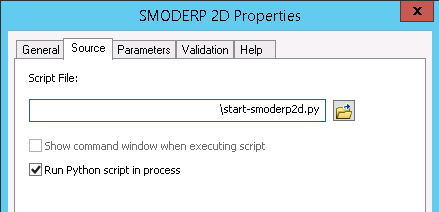
\includegraphics[width=0.75\textwidth]{./img/start-smoderp.png}
    \caption{Ukázka puštění modelu \smod v ArcGIS {\tt toolbox}}
    \label{fig:tbsource}
  \end{figure}  
  
  \begin{figure}
    \begin{tikzpicture}
    \node at (0,0) {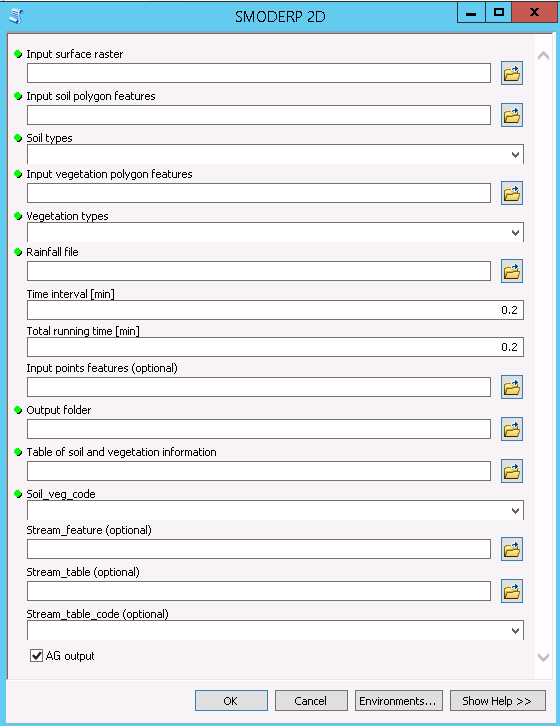
\includegraphics[width=0.75\textwidth]{./img/toolbox.png}};
    
    
    \draw [very thick] (-2.5,5) -- (5,5) node[right] {digitální model terénu sec};
    \draw [very thick] (-2.0,4.3) -- (5,4.3) node[right] {digitální model terénu sec};
    \draw [very thick] (-2.0,3.6) -- (5,3.6) node[right] {digitální model terénu sec};
    \end{tikzpicture}
    \caption{Ukázka parametrů ArcGIS {\tt toolbox}}
    \label{fig:toolbox}
  \end{figure} 
%     \centering
%     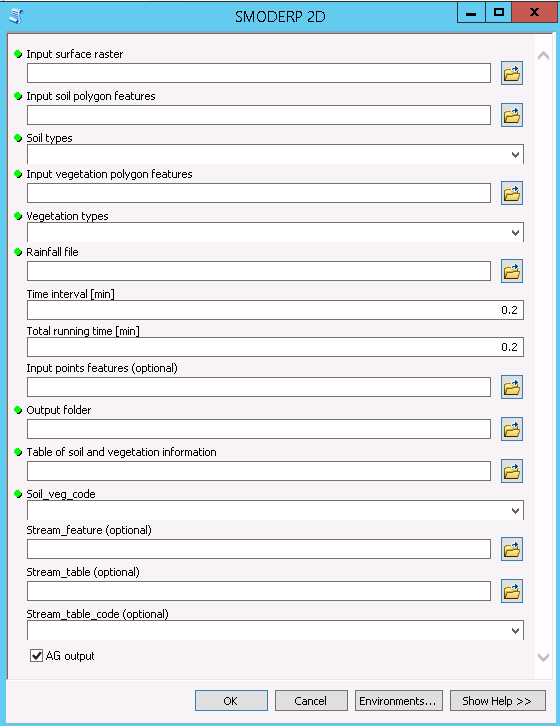
\includegraphics[width=0.75\textwidth]{./img/toolbox.png}
  
  
  
  
  